\chapter{Discussion}

\section{Haptic Performance}
\subsection{From Diagram}
\subsubsection{Motion information}
It is not difficult to discern from the final results that the MotionPerformer system is capable of accurately conveying the direction of movement to users.

In general, individual differences under the 'only-visual' experimental condition are quite minimal. However, in the 'only-haptic' situation, despite having a completely identical system and providing the same haptic feedback for each participant every time, the variances among individuals in response to haptic feedback are noticeably larger than the differences when users obtain movement information visually.

And we will analyze the experimental results from three perspectives - forward and backward displacement movements, left and right rotational movements.

\begin{figure}[h]
\centering
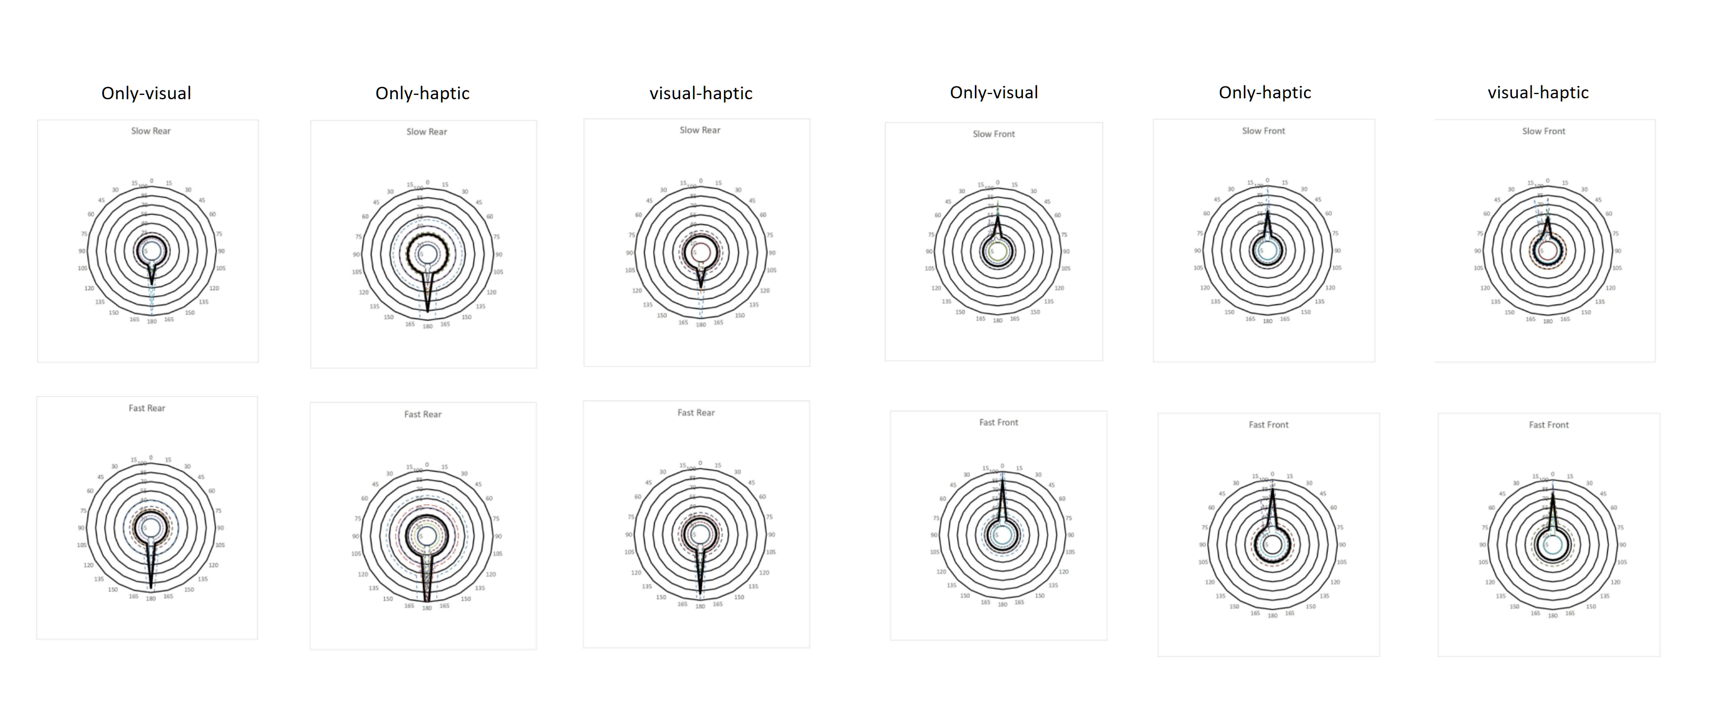
\includegraphics[width=0.8\textwidth]{A_thesis/figures/FrontandRear.png}
\caption{Comparison of displacement direction}
\end{figure}

\newpage
Regarding \textbf{forward and backward displacement movements}, the experimental results under the three different conditions for these two modes of movement are relatively consistent. Notably, user consistency in forward displacement movements is higher than in backward displacement movements. In the backward displacement mode, under the 'only-haptic' condition, users' judgment on displacement distance is significantly greater than in the 'only-visual' condition. Moreover, the judgment variation in high-speed mode is more significant than in low-speed mode, indicating that as speed increases, the perception of backward displacement changes through haptic feedback also intensifies. However, in the combined judgment scenario, the results tend to align more closely with visual judgment.

As for the perception of displacement speed, under the same speed conditions, the speed judged in the 'only-haptic' condition is greater than in the 'only-visual' condition. Yet, in contrast to displacement distance, the rate of increase in speed perception between the low-speed and high-speed modes is nearly the same, with no noticeable difference. After introducing the 'visual-haptic' condition, although the overall trend is the same as the first two situations ('only-visual', 'only-haptic'), it is closer to the 'only-visual' condition compared to 'only-haptic'. Importantly, even though adding haptic feedback results in limited enhancement in displacement variation, it significantly enhances speed perception.

In the comprehensive analysis of displacement direction information, the combined judgment results for forward movement are closer to 'only-visual', while the combined judgment results for backward movement change significantly after introducing haptic feedback. This suggests that incorporating haptic feedback can strengthen users' perception of backward movement. We hypothesize this phenomenon may occur because, in daily life, we experience scenarios involving forward movement far more than backward movement. Furthermore, since the visual direction is always forward, judgments about backward movements require inference from changes in surrounding conditions, making forward movement judgments potentially simpler than those for backward movement. Therefore, our ability to judge forward movement is stronger and more reliant on visual cues. However, the addition of haptic information can enhance our judgment in perceiving backward movement.

\begin{figure}[h]
\centering
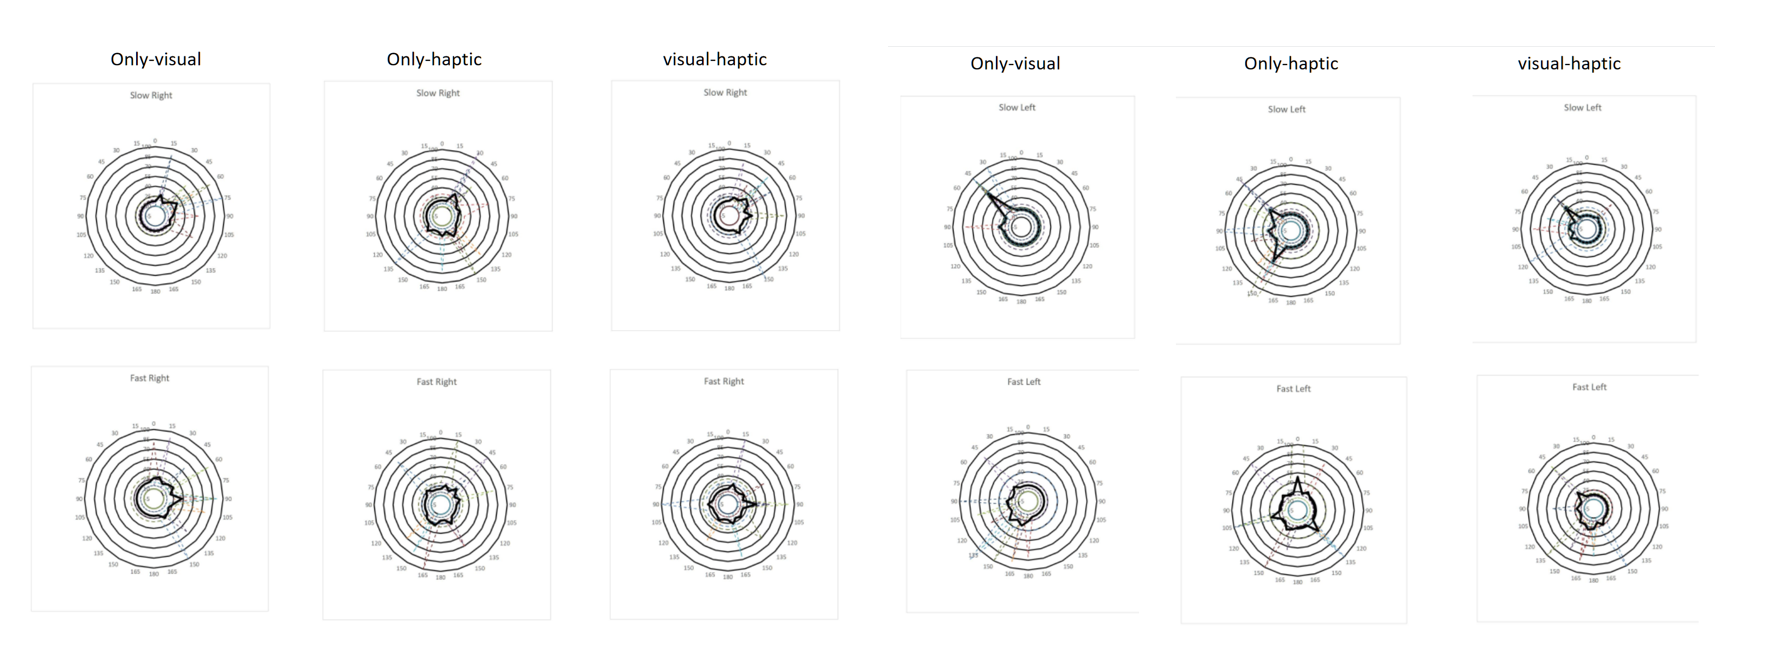
\includegraphics[width=0.8\textwidth]{A_thesis/figures/LeftandRight.png}
\caption{Comparison of rotation direction}
\end{figure}

In terms of left and right rotation, experimental results indicate that haptic feedback significantly enhances users' judgment of rotational angles, but no noticeable improvement is observed in the perception of rotational speed.

For the direction of left-right rotation, the 'only-visual' results are quite concentrated and more accurately represent the actual change in angle. In the 'only-haptic' condition, users' perception of the rotation angle is almost double that of visual judgment. This discrepancy increases in high-speed rotation, to the point that during the experiment, users are unable to discern whether a rotation exceeds 360°. These results suggest that haptic feedback greatly enhances users' perception of changes in rotation angle. However, the specific degree of enhancement cannot be guaranteed by the current results. This is because the rotation speed of the experimental equipment does not accurately correspond to the actual rotation speed, preventing users from establishing their own frame of reference for rotation information in the 'only-haptic' condition. Even in the 'visual-haptic' experimental condition, the introduction of haptic feedback influences users' overall judgment of rotation, reinforcing the aforementioned point. Yet, in terms of rotation angle, the results still align closely with the 'only-visual' condition. This suggests that when significant discrepancies arise between visual and haptic judgments, users still predominantly rely on visual information.

Concerning changes in rotation speed, the introduction of haptic feedback does not noticeably improve speed perception. In the preliminary experiments, users were unable to describe the rotation vector due to excessive speed variation, leading to smaller speed variation ranges in the present experiment. This may be one reason for the lack of significant changes in users' speed perception. Thus, the current experiment's results do not provide a reliable reference for haptic feedback's influence on rotation speed.

Interestingly, the combined judgment after adding haptic feedback is smaller than that of 'only-visual' and 'only-haptic', particularly noticeable in left turns. This indicates that when users receive both visual and haptic information about rotation, their judgment of rotation speed tends to be conservative. However, in the right turn experiment results, introducing haptic feedback did not significantly influence changes in rotation speed. This suggests inconsistent judgment standards when determining left or right rotations.

In summary, regardless of the experimental condition, users judge left turns more accurately than right turns. Even under 'only-visual' conditions, users' judgments of left turns are more focused and precise. This is consistent with the aforementioned point that the judgment conditions or abilities for left and right turns are different, but the specific influencing factors and limitations are not the focus of the current study.

As observed from the results of Experiment 1 Motion Information Diagram, the MotionPerformer can accurately convey the direction of motion to users. Users can perceive speed changes significantly, but the precision of rotation angle information needs improvement. In terms of speed and displacement information, the system can help establish comparisons under different parameters. In other words, the MotionPerformer can provide a reference for mechanics in virtual space, but this reference system is highly subjective. Whether a public, objective mechanical reference coordinate system can be established using the MotionPerformer warrants further consideration and research. Moreover, the MotionPerformer can enhance users' perception of motion information, particularly in backward displacement direction and rightward rotation direction.

\subsubsection{Haptic Sensation of Hand}
During the experiment, users were not forcibly dictated on how to grasp the device. Instead, they were advised to choose a suitable position to minimize the chance of their hands being pinched by the roller part while still being able to feel the haptic feedback.

According to users' descriptions of the areas of their hands that received haptic feedback, which were then visualized and overlapped, results are as follows.

\begin{figure}[h]
\centering

\includegraphics[width=0.5\textwidth]{A_thesis/figures/016.png}
\caption{Results of the hand diagram}
\end{figure}

As the design concept, users primarily felt haptic feedback in areas depending on how they gripped the device, mainly on the back of the third joint of their fingers and a slightly lower position at the center of their palms. 

Interestingly, the index finger had a larger area of haptic feedback compared to other fingers. This isn't just because the index finger is used more often in our daily lives, but also because the natural grasp of the hand is not a horizontal cylinder. Instead, it is a grip where the tail end (little finger) slightly points downward. This point should be taken into consideration in future designs, as a more natural grip could potentially reduce incidents of pinching and enhance the user experience.

In the palm area, the most haptic feedback was not in the center, but mainly in the regions of the flexor digiti minimi brevis muscle (which flexes the little finger) and the flexor pollicis brevis muscle (which flexes the thumb). The reason is similar to what was mentioned earlier. In the natural grip posture, these two areas make contact with the MotionPerformer at certain angles. The haptic feedback provided by these two areas is stronger than the haptic feedback directly received at the center of the palm where it makes contact with the MotionPerformer.

\subsection{From Feedback}
Further evidence supporting the conclusions drawn earlier can be found in users' feedback.

Firstly, users positively affirmed the haptic sensation for directional and angular changes. According to the feedback, users reported a stronger perception of directional vectors compared to rotation vectors through haptic feedback (001). Similarly, the haptic perception of speed information was also found to be more intense than visual perception (002, 007). Although vision can provide more accurate information (002), haptic information proves to be a better judge in certain situations where visual feedback is insufficient, such as during rotation (010).

In comprehensive use scenarios, when both visual and haptic feedback convey the same motion information, users tend to rely more on visual information. However, in situations where visual information is abundant, haptics can provide instant feedback about changes (009), a feature where it distinctly outperforms vision. Several participants also mentioned that adding haptic feedback to the perception system, through the collaboration of vision and haptics, enhances users' overall perception of moving objects in virtual space (002, 004, 008). This allows for a better user experience and a more realistic feeling (001, 005). Generally, the significance of adding the haptic device, MotionPerformer, lies in aiding users to establish a mechanical haptic reference for the self-moving objects in virtual space (005).

Lastly, regarding the reliability of the device, even after optimization, some users still made suggestions for improvements. For example, device latency and judder were mentioned as factors that could reduce immersion during use (004). Incidents of hand pinching were also brought up sometime (003). During testing, it was noticed that pinching incidents occurred more frequently among female testers. Therefore, improvements in device reliability and design are needed in future iterations to achieve a better user experience. Moreover, in terms of experimental design, helping testers establish a reference relationship between vision and haptics prior to the formal test could significantly improve users' perception of accuracy in subsequent processes (008).

\section{User Experience}
\subsection{The Sense of Agency}
In the first eight questions of the questionnaire, the main content was to test whether the device possesses a sense of agency. Four questions (Q1, Q5, Q6, Q7) have a positive impact on the sense of agency, the higher the value, the stronger the sense of agency. The other four questions (Q2, Q3, Q4, Q8) negatively impact the sense of agency, the higher the value, the weaker the sense of agency.

In the analysis process, the Cohen’s d value was calculated to assess the effectiveness of the difference between the two situations in addition to the use of t test for the calculation of statistical differences. The following discussion is arranged from the largest to smallest Cohen's d value.

\begin{figure}[h]
\centering
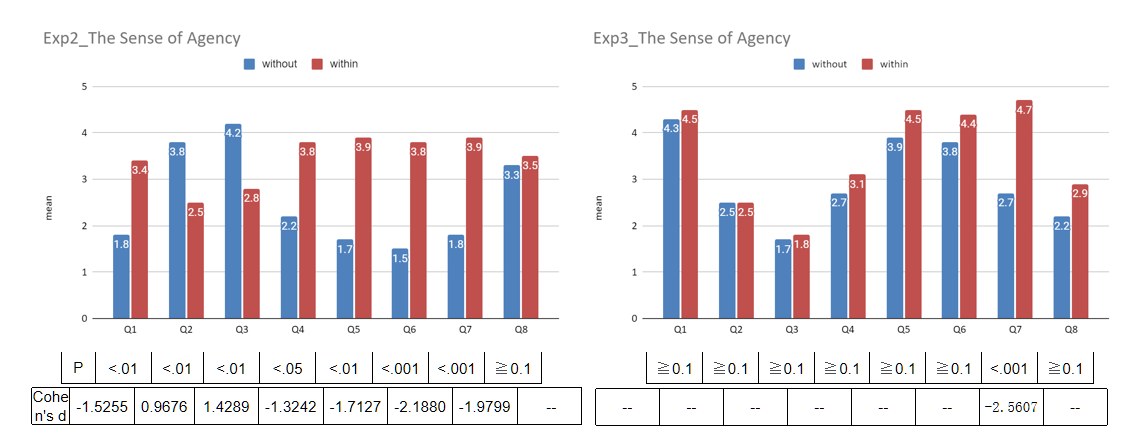
\includegraphics[width=0.9\textwidth]{A_thesis/figures/040.png}
\caption{Data visualization on the sense of agency}
\end{figure}

\subsubsection{Passive Usage Scenarios}
\begin{figure}[h]
\centering
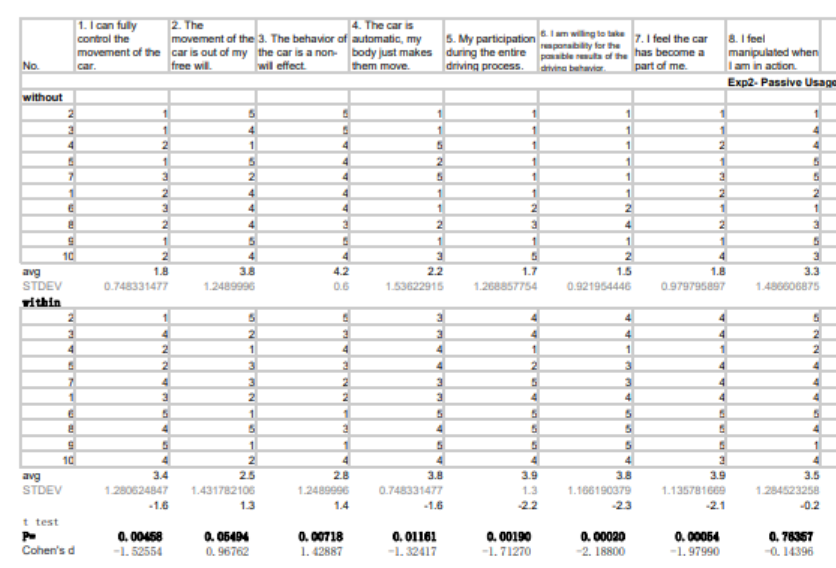
\includegraphics[width=0.8\textwidth]{A_thesis/figures/014-01.png}
\caption{Results on the sense of agency in passive use scenarios}
\end{figure}

In passive/inactive usage scenarios, the use of MotionPerformer greatly enhances users' sense of agency.

Q6: In passive driving situations, users refuse to take any responsibility for the consequences of the system's actions because they don't participate in any driving behaviors. However, after using MotionPerformer, by receiving the motion information of the vehicle, users' trust in the system is strengthened even though they are not involved in the driving process. This means they are more likely to trust the autonomous judgement of automation devices.

Q7: Despite emphasizing that users are in a simulated driving environment before the experiment, they still find it hard to feel that they and the vehicle have become a unity or that they have become the embodiment of the vehicle in the virtual environment. However, MotionPerformer can break the physical self-efficacy. It enhances the conveyance of motion information from automation devices to users, incorporating the automated devices into the users' framework of self. This generates a feeling that the vehicle has become a part of the user's body.

Q5: Before using the device, users do not have a significant sense of involvement, as the ideal situation often doesn't require users to make any actions during smart driving. However, using MotionPerformer greatly enhances users' sense of involvement in the movement process.

Q1: After using the device, users' perception of device control is enhanced. Even in passive usage scenarios, it still gives users a feeling of active control.

Among the negatively impacting parameters, the most significant ones are Q3 and Q4.

Q3: The behavior of the vehicle, which is not controlled by the user, is widely acknowledged in passive usage situations. However, after using MotionPerformer, users' judgement of autonomous actions begins to waver, leading them to question whether their intentions influence vehicle behavior during the driving process.

Q4: This reflects a similar problem. When it is mentioned that the system is automated and that user drives the automated motion behavior, users have a negative attitude in passive usage situations. However, after using MotionPerformer, users begin to acknowledge that even automation devices' movement behaviors can be influenced by the user themselves.

\subsubsection{Active Usage Scenarios}
\begin{figure}[h]
\centering
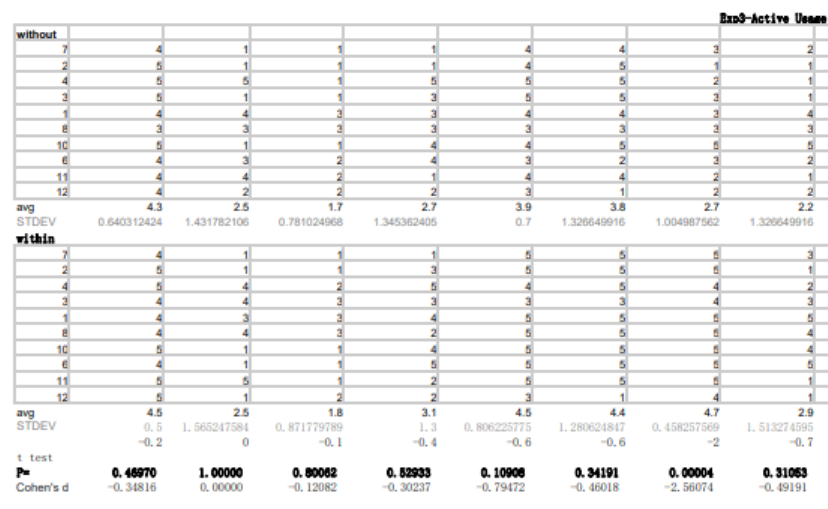
\includegraphics[width=0.8\textwidth]{A_thesis/figures/014-02.png}
\caption{Results on the sense of agency in active use scenarios}
\end{figure}

In active usage scenarios, since users are already independently controlling the vehicle's operation, the overall improvement in the sense of agency is very limited. The largest improvement is in Q7, where users acknowledge that by using MotionPerformer, the vehicle becomes a part of their own body. We believe that this not only enhances the sense of agency in driving but also changes and improves users' identity recognition. It allows users to reconsider the whole system's impact on them from their own cognitive perspective, rather than just from the perspective of an operator or driver.

\subsection{User Experience}

\begin{figure}[h]
\centering
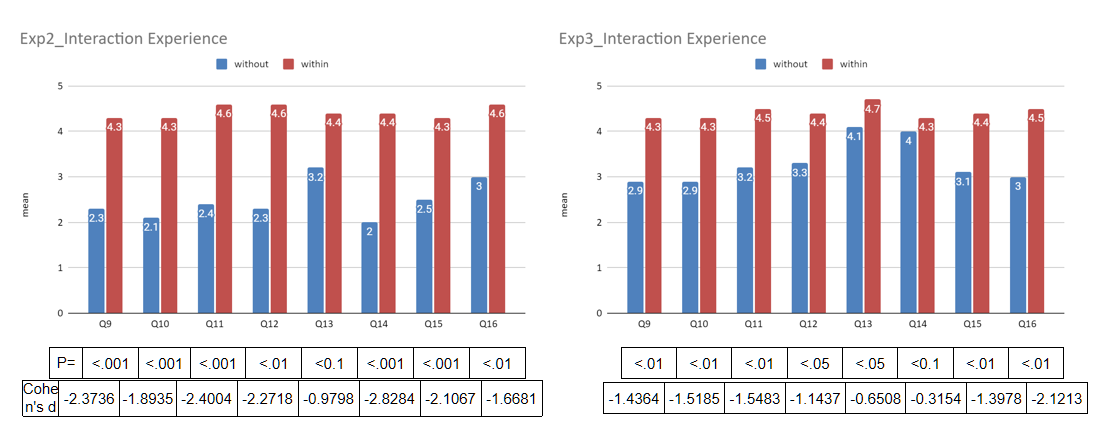
\includegraphics[width=0.9\textwidth]{A_thesis/figures/041.png}
\caption{Data visualization on user experience}
\end{figure}

\begin{figure}[h]
\centering
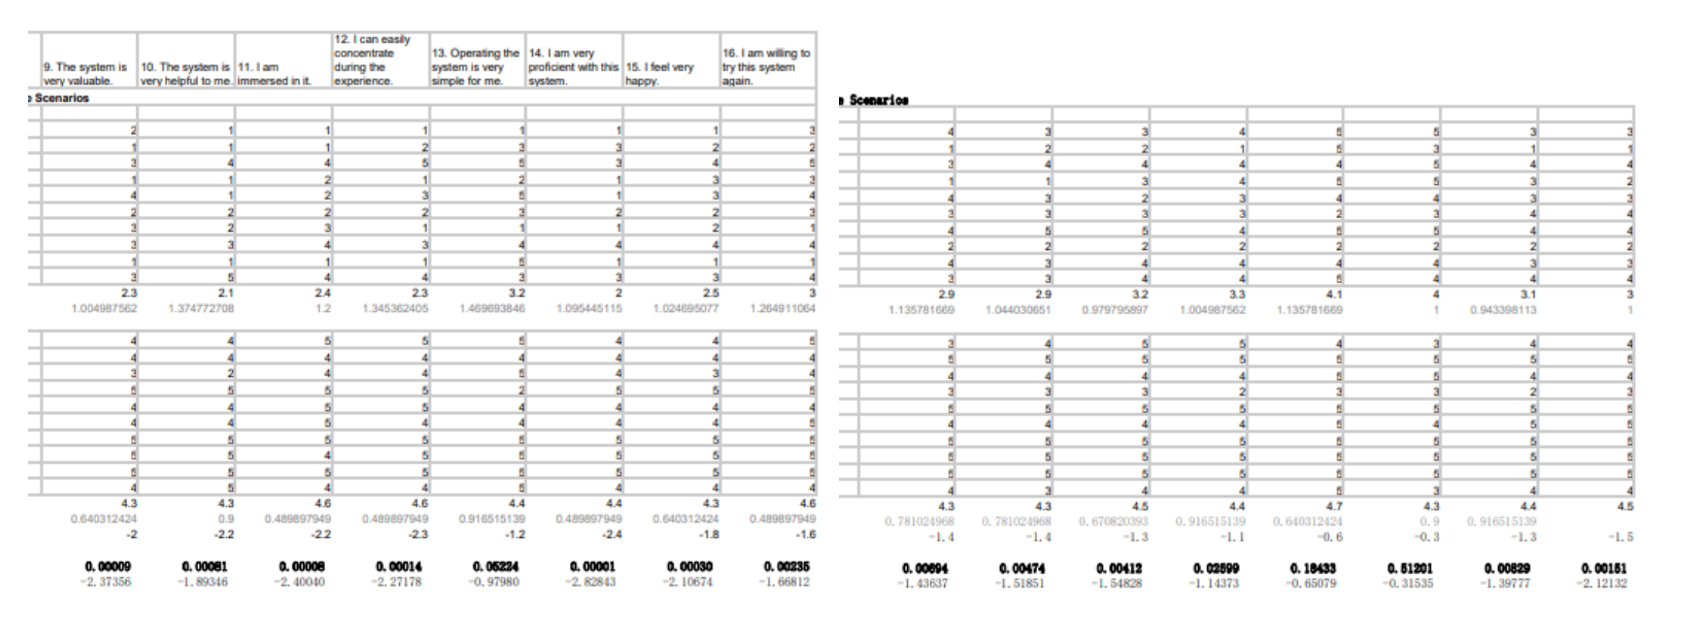
\includegraphics[width=0.95\textwidth]{A_thesis/figures/015.png}
\caption{Results on user experience}
\end{figure}

The last eight questions of the questionnaire mainly test the user's feeling and experience when using the MotionPerformer. In our original hypothesis, we thought that the active scenario might be more popular in terms of user experience, providing a greater experience. However, the results show that after introducing the MotionPerformer haptic system, the enhancement of the passive scenarios is greater than that of the active scenarios.

Q9 and Q10 primarily reflect whether the use of the MotionPerformer system is meaningful to users, and positive feedback was received in both usage scenarios. As previously mentioned by the users in their feedback, introducing MotionPerformer into the automation system helps users gain more information about the device's movement. In interactions with the intelligent system, having more information increases trust in the system. Users can also obtain information through haptic feedback that they didn't get visually.

Q11 and Q12 mainly reflect whether the user's immersion has increased after using the MotionPerformer system. In the passive usage scenario, users' sense of immersion has greatly improved. Feedback also mentioned that after gaining more haptic feedback, users will have more information for judgment. Interactions with the automation device will make users more willing to invest more attention into the operation of the automation system.

Q13 reflects whether the device is easy to control. Although the impact isn't as significant as other areas when combining both scenarios, the system itself is already relatively simple in the case of not using the device, so the improvement is very limited. However, We have reason to believe that in a more complex automation device, MotionPerformer can effectively reduce the complexity of operation.

Q14 is similar but not identical to Q13. Q14 mainly reflects mastery, this aspect mainly reflects the user's grasp and understanding of the entire system in the overall experience. It's worth noting that there is a significant impact difference between passive scenarios and active scenarios in this aspect. In the passive scenario, the effect is extremely significant. Like the improvement of the sense of agency, after receiving the haptic information provided by MotionPerformer, users no longer view the automation device as an independent system. Instead, they start to incorporate the automation device into their self-awareness through sharing haptic information and motion information. Since the acceptance of the device indicates that users will be superior in physical mastery and conceptual understanding compared to situations where haptics are not shared. In contrast to the results o passive scenarios, there is almost no significant improvement in this aspect in active scenarios. We believe that when users can already control the movement of objects, they have started to think from the perspective of the automation system or the pilot. Therefore, when the users has conceptually accepted the device, the improvement brought by MotionPerformer is not very effective.

Q15 and Q16 reflect whether MotionPerformer brings emotional value and enjoyment. Although both scenarios have achieved effective improvement in this aspect, the emotional value obviously has more improvement in the passive usage scenario. This represents that although users are in the interaction with the intelligent system, they would still choose a solution that brings haptic information. As for enjoyment, it's obviously more affected in the active scenario. Whether it's in a simulated driving scenario or a gaming application scenario, MotionPerformer brings rich haptic information, effectively enhancing the user's sense of entertainment.
